\documentclass[10pt,letterpaper]{article}
\usepackage[margin=.82in]{geometry}
\usepackage[T1]{fontenc}\usepackage{lmodern,graphicx,booktabs,amsmath,xcolor,hyperref,xurl,caption,fancyhdr}
\hypersetup{colorlinks=true,urlcolor=teal,linkcolor=teal,pdftitle={Keep cotton quality in a price alert},pdfauthor={James Jean}}
\pagestyle{fancy}\fancyhf{}\fancyhead[L]{\small Cotton quote integrity / Study 30}\fancyhead[R]{\small Independent controlled study}\fancyfoot[C]{\thepage}
\setlength{\headheight}{14pt}\setlength{\parindent}{0pt}\setlength{\parskip}{6pt}\captionsetup{font=small,labelfont=bf,hypcap=false}
\begin{document}
{\small\color{teal} PRICE PIPELINES / QUOTATION IDENTITY\par}
\vspace{8pt}{\LARGE\bfseries Keep cotton quality in a price alert\par}
\vspace{7pt}James Jean \hfill 30 October 2026
\section*{The decision}
A price feed can offer another quality without changing the price of its original quality. Averaging the rows before comparing snapshots can turn that composition change into an alert. This study supplies an inspectable historical controlled replay, a local comparison tool and an implementation exercise for preserving the intended price series.

\textbf{Finding.} At the fixed 2\% threshold, the grade-blind rule raises \textbf{1,757 false alerts in 1,757 zero-change expansion cases} from the later source year. Each case keeps the original quotation unchanged and adds another quality. Comparing the identical original quality removes that composition effect by construction. This is a deterministic identity safeguard, not evidence of live anomaly-detection precision.

\begin{center}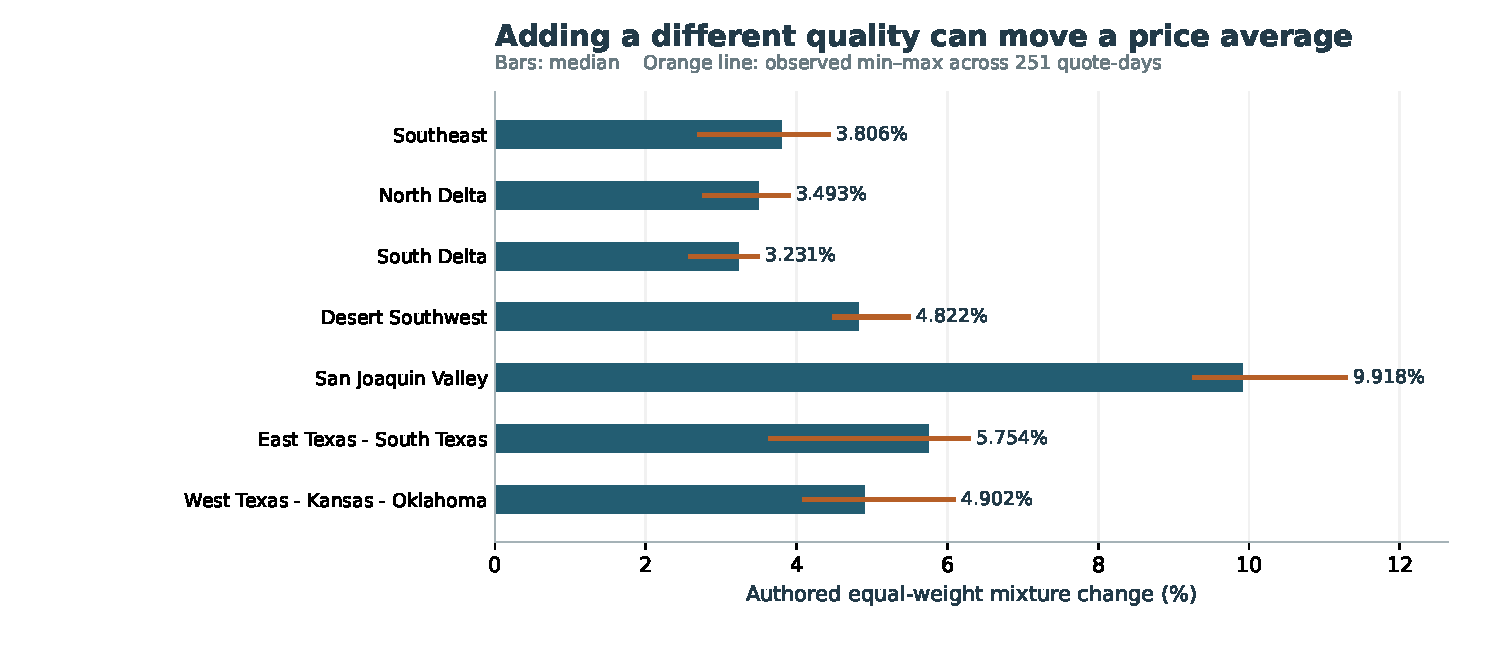
\includegraphics[width=\linewidth]{images/composition_effects.pdf}\end{center}
\captionof{figure}{An authored snapshot adds the historical 31/3/36 quotation to the unchanged 41/4/34 quotation. Equal-weight mean change equals half the relative quality premium. Bars show the median; lines show the minimum and maximum across the 251 later-year quote-days in each market. These are controlled mixture effects, not observed temporal price jumps or uncertainty intervals.}

\textbf{Practical recommendation.} Keep market, units, report date, complete quality definition and other-quality convention in the comparison key. When that identity is missing or conflicting, emit an unavailable result for reconciliation. Live integration still needs source-version mappings, arrival monitoring and shadow evaluation with real failure labels. No financial saving is measured here.
\newpage
\section*{1. What the historical source supports}
The source is USDA Agricultural Marketing Service's public upland price-file archive [1]. Three fixed XLSX objects were captured once after protocol commit \texttt{eb549df}, with request URLs, UTC timestamps, HTTP status, byte counts and SHA-256. The original workbooks stay private and unchanged. Their \texttt{C-L-S} sheets supply date, market, color, leaf, staple, quality difference and physical price. Only the supplied physical spot price in cents per pound enters the comparison; ICE futures, basis points and transaction volumes do not.

The exact source projection retains 12,032 rows for the two planned quality definitions, including US-average rows with an exclusion reason. It contains 10,528 eligible quotation keys and 5,264 paired market/date observations. There are no conflicting or duplicate eligible keys. Each source year has seven native market groups and passes the fixed minimum of 100 paired quote-days in every group.

\begin{center}\begin{tabular}{lrrr}\toprule
Marketing year & Markets & Paired days / market & Total pairs\\\midrule
2022--2023 & 7 & 249 & 1,743 \\
2023--2024 & 7 & 252 & 1,764 \\
2024--2025 & 7 & 251 & 1,757 \\
\bottomrule\end{tabular}\end{center}

\textbf{Quality and geographical identity.} The planned definitions are color 41 / leaf 4 / staple 34 and color 31 / leaf 3 / staple 36. Other factors use the source report's base convention: mike 3.5, 3.6 and 4.3--4.9; strength 27.0--28.9 grams per tex; uniformity 81.0--81.9. The convention describes a quotation grid, not measured attributes of independent bales. Source spot terms are net weight, mixed lots, FOB car/truck including compression and brokerage [2]. Every eligible grid base price agrees exactly with its separate headline-sheet base price after an explicit within-file spelling binding.

\textbf{A format announcement is motivation, not an incident label.} USDA's October 31, 2024 newsletter announces an August 1, 2025 headline quality of 31/3/36 while retaining 41/4/34 [3]. Older reports already list 31/3/35. The one-row-to-two-row transformation below is authored; it does not reconstruct the actual transition or establish that a customer pipeline failed.

\textbf{Recorded integration corrections.} Initial inspection exposed the first 11 data rows of each sheet in the first workbook as well as headers; primary searches exposed some 2024 report values. There is no analyst-blindness or untouched-schema claim. An initial abbreviated-market binding rejected spelled-out grid names; one pre-score correction binds the exact names by source year. Changed Texas-region definitions are retained, not silently pooled. A malformed repeated West Texas label appears outside the target grades and is not repaired. Full workbooks, third-party futures values, source PDFs, contacts and logos are excluded from publication under the stated rights scope [4].
\newpage
\section*{2. Fixed cases and earlier development}
For each eligible pair, let $B>0$ be the original base quotation and $H\geq0$ the alternative quality quotation. The old snapshot has $B$. The new snapshot has either the same quality alone or that quality plus $H$. Apply an authored uniform multiplier $1+s$ to the new quotations, with
\[
s\in\{0,-0.10,-0.05,-0.02,+0.02,+0.05,+0.10\}.
\]
When the original identity remains, the matched change is exactly $s$. With an added quality, the grade-blind change is
\[
g_{\rm blind}=\frac{(B+H)(1+s)}{2B}-1.
\]
At $s=0$ it is $(H/B-1)/2$: a mixture effect even though $B$ is unchanged. Exact fractions use native XLSX decimal tokens, preserving extra source digits rather than rounding prices to force threshold agreement.

An alert means $|g|\geq t$ for each fixed $t\in\{0.01,0.02,0.05\}$; the authored label is $|s|\geq t$. All six rule/threshold combinations remain retained. Thresholds are proposed sensitivity choices, not learned or optimized limits. The equally enumerated grid has positive-label shares 6/7 at the 1\% and 2\% thresholds and 4/7 at 5\%. These are authored class shares, not natural market-anomaly prevalence.

Development uses 1,002 paired days in Southeast and North Delta from the two earlier files. Across two expansion states, seven signed changes, three identity modes, two rules and three thresholds, it enumerates 252,504 cases. Independent formulas check 3,584,316 exported conditions. The table below retains all fixed thresholds for normal-identity, added-quality snapshots; full exports also retain no-expansion, signed-change, market, month and failure-mode breakdowns.

\begin{center}\small\begin{tabular}{llrrrrrr}\toprule
Rule & $t$ (\%) & TP & FP & TN & FN & Precision (\%) & Recall (\%)\\\midrule
Blind & 1 & 5,011 & 1,002 & 0 & 1,001 & 83.34 & 83.35 \\
Matched & 1 & 6,012 & 0 & 1,002 & 0 & 100.00 & 100.00 \\
Blind & 2 & 5,010 & 224 & 778 & 1,002 & 95.72 & 83.33 \\
Matched & 2 & 6,012 & 0 & 1,002 & 0 & 100.00 & 100.00 \\
Blind & 5 & 3,006 & 16 & 2,990 & 1,002 & 99.47 & 75.00 \\
Matched & 5 & 4,008 & 0 & 3,006 & 0 & 100.00 & 100.00 \\
\bottomrule\end{tabular}\end{center}

Precision is TP/(TP+FP), and recall among emitted comparisons is TP/(TP+FN). An empty denominator is unavailable. Abstentions are recorded separately and never become correct negatives. No probability or calibration claim is made. There is no fitted model, candidate selection or training seed. The broader historical anomaly-forecasting proposal remains unexecuted context.
\newpage
\section*{3. Later year and additional markets}
Dependency-freeze commit \texttt{8b0bf69} binds 37 files before any later case summary: protocol, native source bindings, source/input evidence, comparison and checking code, fixtures and development exports. The later application uses all seven 2024--2025 native markets, adding five market groups to the two used in development. Earlier full-source rows were visible for qualification. This is a frozen deterministic application with disclosed source exposure, not a prospective or analyst-blind anomaly trial.

The full later grid has 442,764 authored cases; independent reconstruction checks 6,284,563 exported conditions. Added-quality snapshots with the original identity present give:

\begin{center}\small\begin{tabular}{llrrrrrr}\toprule
Rule & $t$ (\%) & TP & FP & TN & FN & Precision (\%) & Recall (\%)\\\midrule
Blind & 1 & 9,466 & 1,757 & 0 & 1,076 & 84.34 & 89.79 \\
Matched & 1 & 10,542 & 0 & 1,757 & 0 & 100.00 & 100.00 \\
Blind & 2 & 8,340 & 1,757 & 0 & 2,202 & 82.60 & 79.11 \\
Matched & 2 & 10,542 & 0 & 1,757 & 0 & 100.00 & 100.00 \\
Blind & 5 & 4,829 & 2,398 & 2,873 & 2,199 & 66.82 & 68.71 \\
Matched & 5 & 7,028 & 0 & 5,271 & 0 & 100.00 & 100.00 \\
\bottomrule\end{tabular}\end{center}

\begin{center}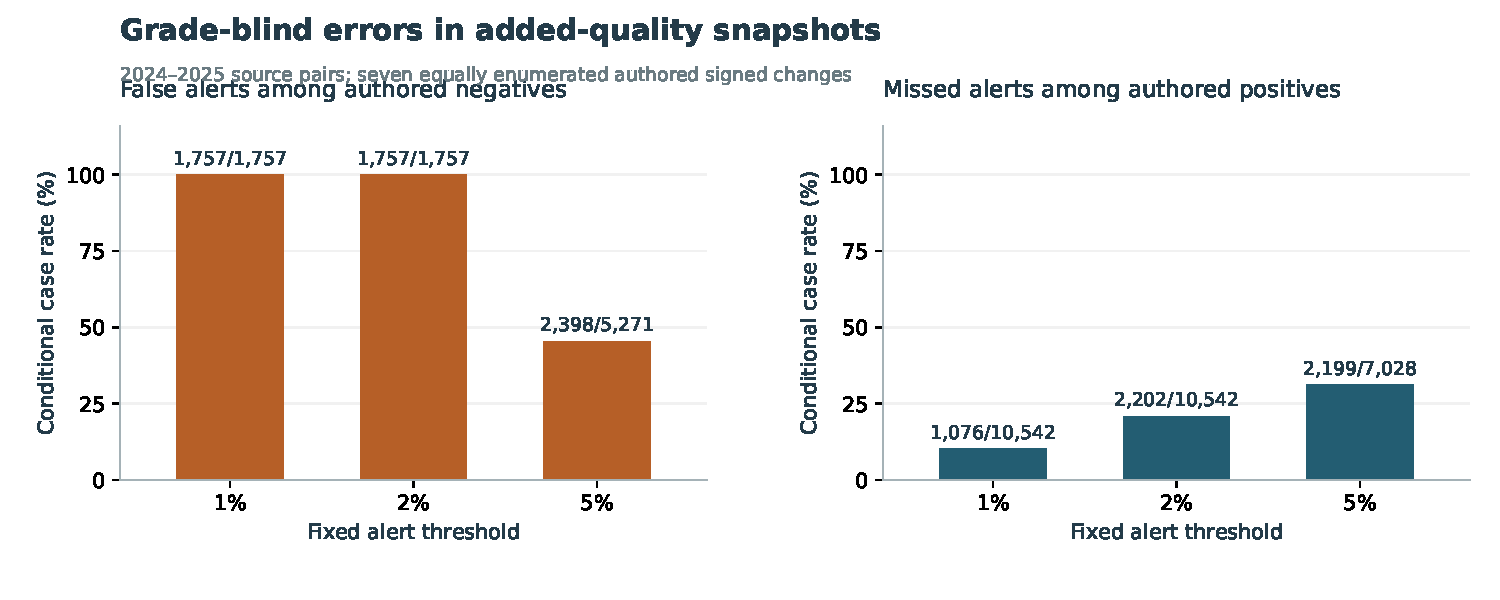
\includegraphics[width=\linewidth]{images/alert_errors.pdf}\end{center}
\captionof{figure}{Grade-blind errors conditional on the authored normal-identity, expansion grid. Denominators change with the truth threshold. The matched rule has zero false and missed alerts in these cases because it compares the unchanged identity under the same multiplier used to construct the truth. That finite property does not establish live anomaly recognition.}

At 2\%, the grade-blind rule also misses 2,202 authored positive cases. A quality premium can offset a negative same-quality change. Both rules give the exact authored change without expansion, as the arithmetic requires. No threshold is retrospectively chosen to improve the story, and no causal, significance, independent-replication or market-generalization claim follows from these counts.
\newpage
\section*{4. Missing identity changes the decision}
Two additional fixed failure modes remove the base quote or change its quality identity. The changed-identity case explicitly uses an authored different staple; it does not invent a USDA crosswalk or assert physical equivalence. The truth multiplier remains recorded for diagnosis, but same-quality identification is unavailable.

\begin{center}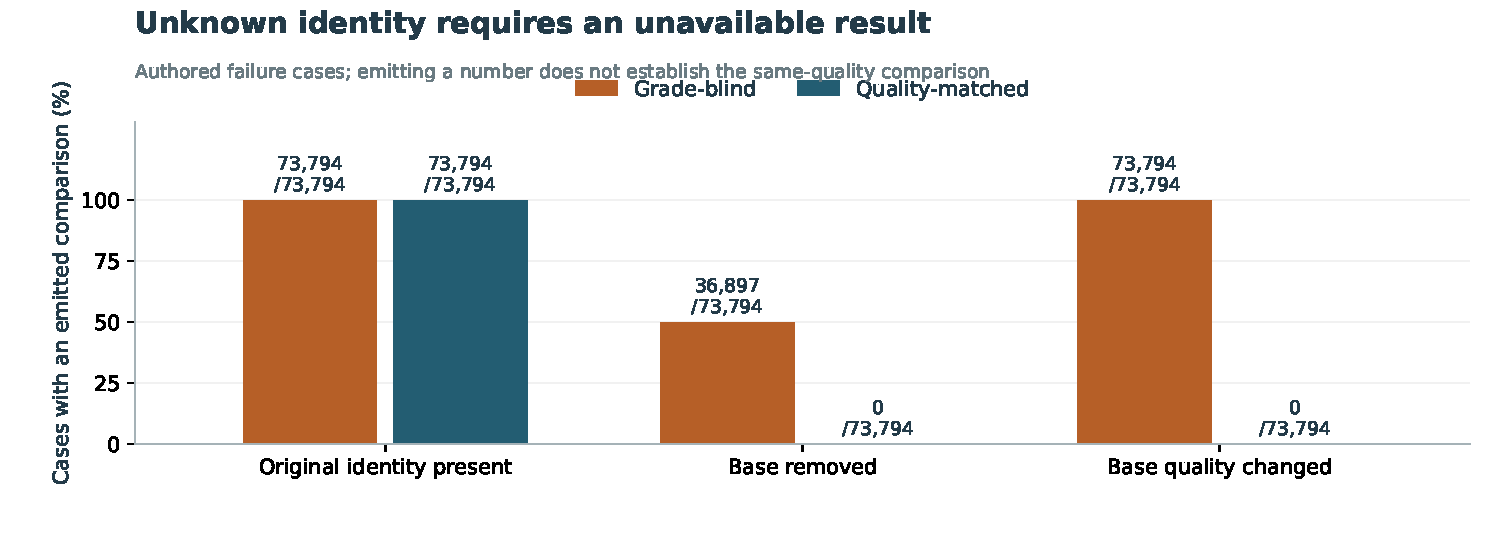
\includegraphics[width=\linewidth]{images/identity_coverage.pdf}\end{center}
\captionof{figure}{Coverage across both expansion states, all signed changes and all thresholds in the later source year. Removing the base leaves an empty snapshot without expansion, so the blind rule also abstains in half those cases. When another quality remains or the base identity is altered, a blind numerical output does not establish that the original quality was compared. Matched-rule abstention is required by the key guard; it is not a predicted negative or measured anomaly-detection success.}

\textbf{Implementation exercise.} The repository supplies authored JSON snapshots with one base quote at 80 and an added quote at 88. The blind mean becomes 84, an exact 5\% change, while the base remains unchanged. The local CLI defaults to the matched rule and reports an exact fractional change, alert or unavailable reason. The exercise asks the reader to implement the guard before consulting the reference solution.

The comparison requires market, source date, unit, other-quality convention and a nonempty original quality. It rejects mismatched common identity, nonpositive baseline, invalid prices, conflicting matched copies, binary-float inputs without native decimal tokens and missing original price. The 28 finite fixtures cover these failure modes and exact threshold boundaries. They do not establish universal correctness or production readiness.

\textbf{For a real feed.} Confirm versioned quality definitions and published units before loading a price series. Preserve the native quote and source arrival time, record a rejection reason instead of silently coercing missing to zero, and keep series changes explicit. Shadow-test actual report updates and independently labeled incidents before assigning alert precision or choosing an operating threshold. This study provides that local comparison boundary and a controlled diagnostic, without a deployed monitoring service or measured customer benefit.
\newpage
\section*{5. Evidence, limits and next step}
The source checks reconcile 360,999 original-cell/native-token conditions with independent Openpyxl and stdlib OOXML readers. SQLite/Decimal independently verifies 99,416 source-key, date, unit and coverage conditions. Figure checks compare source values with actual SVG geometry and exported hashes. A public offline replay starts from the committed minimal quotation projection; repeating original-cell reconciliation additionally requires the recorded private workbook snapshots. Network recapture is not presented as the same historical byte version.

Runtime receipts preserve the byte hashes of their as-run exports. Git text canonicalization changes JSON line endings; supporting container checks distinguish those recorded runtime bytes from current canonical bytes, preserving the frozen numerical receipt rather than replacing it. Replay compares exact CSV fields and JSON content in separate output directories and verifies that all frozen originals remain unchanged. This representation distinction does not alter a source token, case, threshold or numerical conclusion.

\textbf{Limitations.} USDA quotations are reported market-grid values, not individual transactions, independently sampled bales or realized purchase prices. Dates and qualities share market information; authored cases repeatedly reuse those quotations. Equal case enumeration and two-row averaging are declared assumptions. No volume weighting, incident probability, confidence interval, forecast, fitted anomaly model or causal price-change attribution is established. Market names and geographical definitions differ across source years and are retained explicitly. The identity safeguard is elementary and deterministic; no new-estimator, scientific-priority or peer-review claim is made.

\textbf{Next evidence needed.} Use an authorized live feed in shadow mode, preserve exact report versions and arrivals, obtain independent failure labels, and measure reconciliation workload plus false and missed alerts under the real incident mix. Choose thresholds against that decision context. This historical controlled replay supplies neither a financial return estimate nor evidence that the published 2025 transition actually caused pipeline errors.

\section*{Sources and reproducibility}
\small
[1] USDA AMS, Historical Upland Prices. Three named 2022--2023, 2023--2024 and 2024--2025 price workbooks. URLs and exact capture hashes are in the source receipt. \url{https://apps.ams.usda.gov/Cotton/HistoricalUplandPrices/}

[2] USDA AMS, Daily Spot Cotton Quotations, May 10, 2024, Vol. 106 No. 197. Archived report defining spot terms, physical-price units and other-quality base factors. \url{https://downloads.usda.library.cornell.edu/usda-esmis/files/gb19f580q/t722jz84c/3t947d25s/CNDDSQ.PDF}

[3] USDA AMS, Cotton and Tobacco stakeholder newsletter, October 31, 2024, Market News update. \url{https://content.govdelivery.com/accounts/USDAAMS/bulletins/3bd797d}

[4] USDA, Policies and Links, Digital Rights and Copyright. Government-information attribution with marked third-party exceptions; source originals and ICE values excluded. \url{https://www.usda.gov/about-usda/policies-and-links}

Code, source projections, fixed cases, complete metrics, CLI and exercise: \url{https://github.com/S3R3Bii/cotton-grade-price-alerts}. Independent program manuscript; no formal-submission project is included.
\end{document}
